\DiaryEntry{Primes, Factor Distribution}{2020-11-16}{Number Theory}

In this entry we show some results how the factors of random numbers are distributed.

We consider $10.000$ integers chosen uniformly from the interval $[10.000 ; 100.000]$ and factor them. The following Figure shows the number of factors each has. Note that we count \emph{all} factors; e.g. $8 = 2^3$ has $3$ factors.

\begin{figure}[H]
    \centering
    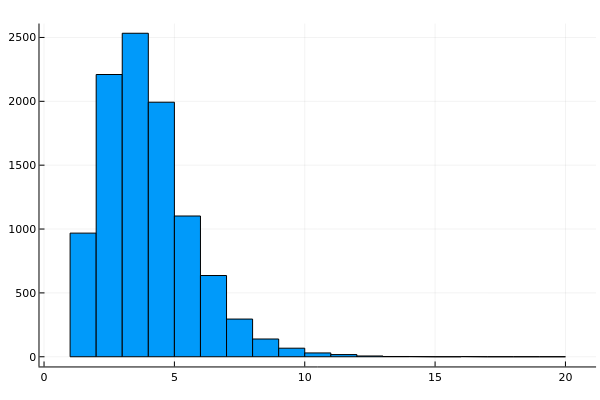
\includegraphics[scale=0.5]{images/primes_03_01.png}
\end{figure}


We see $\approx 1000$ primes (as numbers having one factor) which is rather high. Most often are $3$ factors (about $2500$ numbers). More than $10$ factors is very unlikely; the curve drops off rather quickly.

We next consider $10.000$ random numbers from the interval $[10.000 ; 100.000]$ and show the number of factors in the Figure below.

\begin{figure}[H]
    \centering
    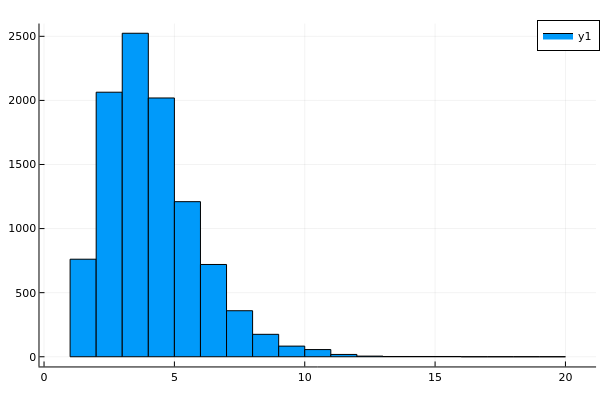
\includegraphics[scale=0.5]{images/primes_03_02.png}
\end{figure}


Nothing fundamentally has changed; there are fewer primes, but the peak with $3$ factors is still here and having more than $10$ factors is still unlikely (although a bit more likely than in the previous setup).

Now we consider the prime density in the following Figure; e.g. the data point $0.070435$ at $10^6$ means that the prime density is $0.07$ in the interval $[10^6; 2 \cdot 10^6]$; i.e. there are $0.070435 \times 10^6 = 70435$ primes in this interval. It can be seen that the number of primes is decreasing with larger numbers.

\begin{figure}[H]
    \centering
    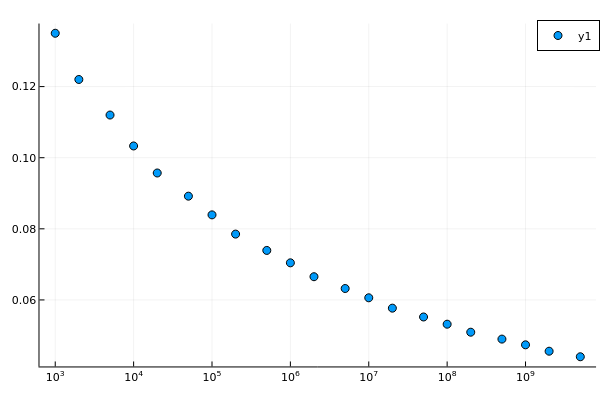
\includegraphics[scale=0.5]{images/primes_03_03.png}
\end{figure}


The Julia script is \href{https://github.com/ClemensFMN/JuliaStuff/blob/master/NumberTheory/prime_count.jl}{here}. Note that it counts \emph{all} primes and does \emph{not} use a random measurement of prime densities. Counting all primes in the last interval ($5$ billion to $10$ billion) is quite CPU consuming and took about one minute.



%%% Local Variables:
%%% mode: latex
%%% TeX-master: "journal"
%%% End:
